\documentclass[10pt,a4paper]{article}
\usepackage[utf8]{inputenc}
\usepackage[T1]{fontenc}
\usepackage{graphicx}
\usepackage{wrapfig}
\title{Examining Muon Scattering Tomography for Imaging Nuclear Materials}
\author{Aditya Patwardhan and Konstantin Borozdin}
\begin{document}
\maketitle

\section{Abstract}
    This paper evalutes muon scattering tomography as an indirect method of detecting nuclear materials inside a bunker. Data from a Monte Carlo simulation in Geant4 is analyzed using the distribution of scattering angles and the percentage of material detected. The simulation is run with cubes of iron and plutonium and various image resolutions. It was found that a detector geometry could be calibrated to produce images of nuclear material with above 80\(\%\) and as high as 99\(\%\) accuracy.
    
\section{Introduction}
    Nuclear nonproliferation is an important challenge in the world today. While direct inspection and imaging methods can be used for many types of nuclear material control, non-proliferation requires the method used to not reveal sensitive information like the design of a nuclear warhead \cite{international2022iaea}. Furthermore, nuclear material is often shielded. This creates the need for indirect methods of monitoring the amount of nuclear material in a facility. One proposed method for indirect monitoring is muon scattering tomography.
	
\section{Background}
    
    Muons are negatively charged fundamental particles produced by cosmic ray interactions with the Earth's atmosphere. The muon flux at sea level is about 1 muon/cm$^2$ per minute \cite{doeexplainsmuons}. The Coulomb scattering (scattering due to interacting with positively charged nuclei) of muons can be used to image materials. When muons pass near high-Z elements (elements with high atomic numbers), such as radioactive elements, they scatter more than when they pass near low-Z elements \cite{international2022iaea}.

    There are multiple algorithms which reconstruct images from muon scattering data. A simple but effective algorithm for image reconstruction is the point of closest approach (PoCA) algorithm \cite{international2022iaea}, which approximates a single point of scattering by finding the closest encounter of muons' trajectories when entering and exiting the detector, using the vector perpendicular to both the enter and exit trajectories. Using the point of closest approach, the scattering angle of the muon is computed. Given a trajectory vector A of the muon entering the detector and a vector B of the muon exiting the detector, the scattering angle of the muon is given by the formula
    \begin{equation}
        S(A ,B) = acos\left(\frac{A \cdot B}{|A||B|}\right).
    \end{equation}
    Other image reconstruction algorithms include Maximum Likelihood Expectation Maximization (MLEM), which uses multiple images to find the likely location of the material, and Angle Statistics Reconstruction (ASR) \cite{international2022iaea}.

\section{Methods}
\subsection{Setting Up the Simulation}
    A Monte Carlo simulation in the Geant4 library \cite{AGOSTINELLI2003250},\cite{ALLISON2016186},\cite{1610988} was used to simulate the experiment. The simulation code was based off of the Muons4Peace project \cite{adatz273muons4peace}, but written in Python 3, which was made possible by the geant4-pybind binding for Geant4 in Python \cite{haraldgeant4_pybind}. Muons were generated in a half-sphere generation plane using the EcoMug (Efficient COsmic MUon Generator) library \cite{pagano2021ecomug}, for which a Python binding of the EcoMug class was written using the Pybind11 library \cite{pybind11}.

    A four-layered detector (two upper layers to detect the trajectory of the muon when entering, and two lower layers to detect the exit trajectory) is used. Each layer is a plastic scintillator of thickness 5 mm, which was found to be an optimal scintillator thickness \cite{park2023development}. The upper and lower detectors are placed 0.8 meters apart. Placed between the upper two and lower two layers is a cube of either iron or plutonium (depending on the simulation being run).

\subsection{Evaluating the Results}
    The results were evaluated based on the accuracy of the images created, in terms of the scattering angles of the muons passing through the material, and the amount of material detected. For image reconstruction, the point-of-closest-approach (PoCA) algorithm is used and only points with scattering angles of at least 1.5 degrees are considered. Finally, the simulation data used to create images is divided into voxels (3-dimensional pixels) of a set side length.

    The accuracy of the image in terms of the amount of material detected is evaluated according to an imaging accuracy score, given by the percentage of voxels that are overlapping between the sets of voxels in the correct and simulated image combined. As an equation, this is
    \begin{equation}
        A(C, S) = 100 \cdot \frac{2 \cdot |C \cap S|}{|C| + |S|}
    \end{equation}
    where C is the correct set of voxels to be imaged and S is the set of voxels imaged by the results of the simulation.

    Furthermore, to remove voxels of falsely-detected material and create more accurate images, points of scattering near the plastic scintillators are discarded, then voxels are filtered according to the function
    \begin{equation}
        F(n, s) = 0.00006 \cdot n \cdot \left(\frac{s}{25}\right)^3, 
    \end{equation} 
    where F represents the number of muon scattering points (points of closest approach) that must be in each voxel (3D pixel) as a function of the number of muons used (n), and the millimeter side length of a voxel (s) for image reconstruction. The filter function must be proportional to n because the number of muons per unit of volume increases linearly with the number of muons used. It must also be proportional to $s^3$ since assuming an even muon distribution (considering all scattering angles,) the number of muons in a voxel grows proportionally to the volume of the voxel.

    The accuracy in terms of the scattering angle was evaluated by comparing the average scattering angle among the voxels of the images of iron and plutonium. This is computed for differing voxel side lengths with a constant number of muons.

\section{Results}
\noindent
\begin{table}[!ht]
    \centering
    \begin{tabular}{|l|l|l|}
    \hline
        Voxel Side (mm) & Accuracy Score Fe (\(\%\)) & Accuracy Score Pu (\(\%\)) \\ \hline
        1 & 0.19 & 0.31 \\ \hline
        2 & 1.57 & 2.48 \\ \hline
        3 & 4.79 & 7.46 \\ \hline
        4 & 10.46 & 15.66 \\ \hline
        5 & 15.90 & 23.22 \\ \hline
        6 & 22.57 & 31.41 \\ \hline
        8 & 29.46 & 38.76 \\ \hline
        10 & 31.28 & 38.21 \\ \hline
        12 & 64.02 & 80.52 \\ \hline
        15 & 73.39 & 85.25 \\ \hline
        20 & 71.43 & 86.61 \\ \hline
        24 & 73.10 & 99.19 \\ \hline
        30 & 72.00 & 91.53 \\ \hline
        40 & 54.05 & 98.11 \\ \hline
        60 & 66.67 & 66.67 \\ \hline
        120 & 0.00 & 0.00\\ \hline    
    \end{tabular}
    \centering
    \caption{Accuracy Score (\(\%\)) vs Voxel Side Length (mm)}
    \begin{tabular}{|l|l|l|}
    \hline
        Voxel Side (mm) & Scattering Angle Fe (°) & Scattering Angle Pu (°) \\ \hline
        1 & 4.39 & 5.28 \\ \hline
        2 & 4.38 & 5.27 \\ \hline
        3 & 4.38 & 5.26 \\ \hline
        4 & 4.37 & 5.24 \\ \hline
        5 & 4.36 & 5.20 \\ \hline
        6 & 4.35 & 5.15 \\ \hline
        8 & 4.32 & 5.01 \\ \hline
        10 & 4.27 & 4.78 \\ \hline
        12 & 4.58 & 6.17 \\ \hline
        15 & 4.07 & 5.55 \\ \hline
        20 & 3.73 & 5.13 \\ \hline
        24 & 3.68 & 5.08 \\ \hline
        30 & 3.49 & 4.99 \\ \hline
        40 & 3.42 & 4.80 \\ \hline
        60 & 3.48 & 5.19 \\ \hline
    \end{tabular}
    \caption{Average Scattering Angle (°) vs Voxel Side Length (mm)}
\end{table}

\begin{wrapfigure}{r}[\(\)]{0.5\textwidth}
\centering
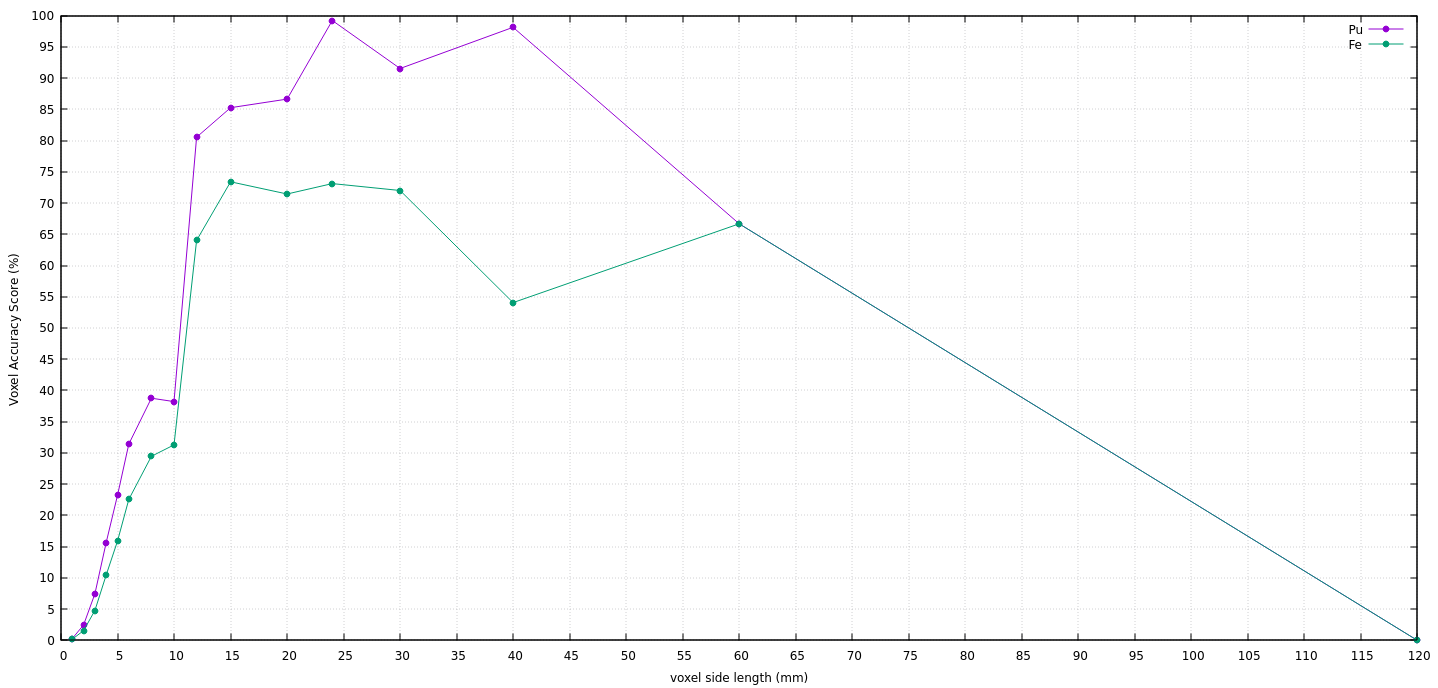
\includegraphics[width=0.5\textwidth]{images/smaller voxel accuracy score vs side len.png}
    \caption{Voxel Accuracy Score (\(\%\)) vs Resolution (mm)}
\end{wrapfigure}

\noindent The first experiment conducted found the accuracy score for voxel detection for imaging a cube of side length 120mm of iron and plutonium using 200000 muons, with differing voxel side lengths that are factors of 120mm (so that the cube can be divided into voxels evenly). The maximum accuracy score was 73.39\(\%\) for iron with a resolution of 15 mm voxels, and 99.19\(\%\) for plutonium with a resolution of 24 mm. As iron has a lower atomic number than plutonium, less of it was detected. The decline in voxel detection accuracy after the peaks can be explained by the filtering function, but it makes sense that the accuracy increases until those peaks as the voxels get larger and the resolution less clear.


\begin{wrapfigure}{l}{0.5\textwidth}
\centering
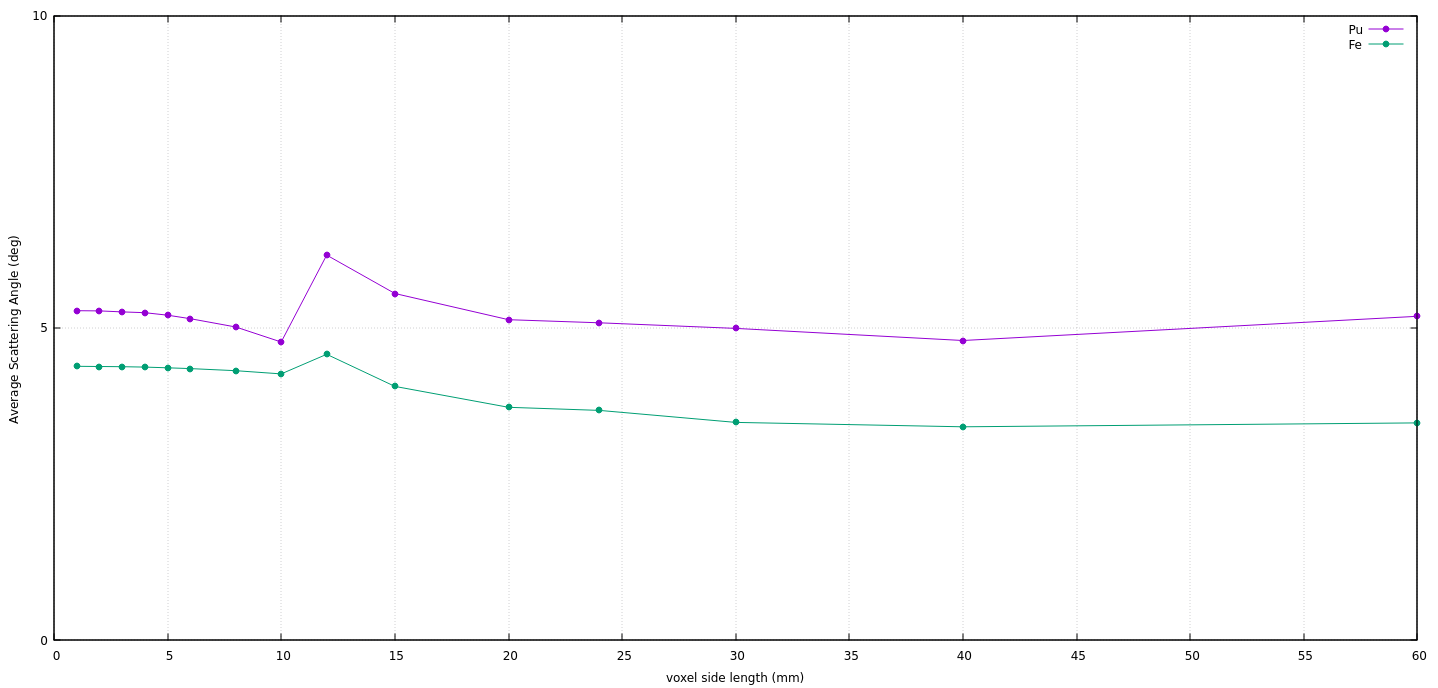
\includegraphics[width=0.5\textwidth]{images/smaller avg scattering angle vs voxel side length.png}
    \caption{Average Scattering Angle (°) vs Resolution (mm)}
\end{wrapfigure}
    The second experiment had the same geometry as the first but found the average scattering angle instead of the accuracy score of voxel detection. As expected, plutonium has a higher scattering angle than iron regardless of voxel size, and for voxels with a side length greater than 10mm, the scattering angle average changes significantly as the accuracy improves. However, the average scattering angle decreases afterwards, which indicates points with higher scattering angles getting represented with fewer voxels and being averaged with lower scattering angles as the voxel size increases.

\section{Acknowledgements}
    We would like to thank the Institute for Computing in Research for providing this opportunity.

\bibliographystyle{ieeetr}
\bibliography{citation}
\end{document}